\documentclass{article}
\usepackage{graphicx}
\usepackage{float}
\usepackage{subcaption}
\usepackage{amsmath}
\usepackage[square, numbers]{natbib}
\bibliographystyle{unsrtnat}
\usepackage[colorlinks=true, allcolors=blue]{hyperref}

\bibliographystyle{alpha}

\title{Information Theory \\ \large Problem Set 06 - Dependent Random Variables}
\author{Luís Felipe Ramos Ferreira}
\date{\href{mailto:lframos\_ferreira@outlook.com}{\texttt{lframos\_ferreira@outlook.com}}
}

\begin{document}

\maketitle

\begin{enumerate}
	\item \begin{enumerate}
		      \item \(H(X, Y)\) is the joint entropy of \(X\) and \(Y\). It means how much information, on average, each of the joint outcomes carries. On other words, is the expected value of information of the joint outcomes from ensembles \(X\) and \(Y\).
		            \[H(X, Y) = \sum_{xy \in \mathcal{A}_x\mathcal{A}_y} P(x, y) log \frac{1}{P(x, y)}\]
		      \item \(H(X | Y)\) is the conditional entropy of \(X\) given \(Y\). It represents the average information infomration content of \(X\) given each \(y \in \mathcal{A}_y\).
		            \[H(X | Y) = \sum_{xy \in \mathcal{A}_x\mathcal{A}_y} P(x, y) log \frac{1}{P(x | y)}\]
		      \item \(I(X, Y)\) is the mutual information between \(X\) and \(Y\). It is the average reduction of uncertainty gain of information about \(X\) when learning the values of \(Y\), or vice-versa, since the mutual information is symmetric.
		            \[I(X; Y) = H(X) - H(X | Y) \]
		      \item \(I(X: Y | Z)\) is the conditional mutual information between \(X\) and \(Y\) given \(Z\). It is the amount of information you gain about \(X\) when you learn about \(Y\) given that the ensemble \(Z\) is known.
		            \[I(X; Y | Z) = H(X | Z) - H(X | Y, Z)\]
	      \end{enumerate}

	\item \begin{enumerate}
		      \item The chain rule for entropy states that:
		            \[H(X_1, X_2, \dots, X_n) = \sum_{i=1}^{n} H(X_i | X_1, \dots, X_{i-1})\]
		      \item The chain rule for mutual information states that:
		            \[I(X_1, X_2, \dots, X_n; Y) = \sum_{i=1}^{n} I(X_i; Y | X_1, \dots, X_{i-1})\]
		      \item The data-processing inequality (DPI) staets that, if \(X \rightarrow Y \rightarrow Z\) is a Markov Chain, i. e. \(p(x, y, z) = p(x) p(y | x) p(z | y)\) for all values in the ensembles, then \(I(X;Z) \leq I(Y;Z)\).
		            In general words, the inequality states that post-processing cannot create information, i.e, the amount of information you have after post-processing data is at most equal to the amount of information before the processing.
	      \end{enumerate}

	\item
	      \begin{itemize}
		      \item \(H(X, Y)\)
		            \[H(X, Y) = H(U, V, V, W) = H(U) + H(V | U) + H(V | U, V) + H(W | U, V, V)\]
		            \[H(X, Y) = H(U) + H(V) + 0 + H(W) = H_u + H_v + H_w\]

		            \(H(V | U) = 0\) since \(U\) and \(V\) are independent, and \(H(V | U, V)\) is obviously zero cause no information is gained.

		      \item \(H(X | Y)\)
		            \[H(X | Y) = H(U,V | V, W) = H(U | V, W) + H(V | V, W, U) = H(U) + 0 = H(U) = H_u\]

		            \(H(U | V, W) = 0\) since \(U, V, W\) are independent and \(H(V | V, W, U)\) is obviously zero.

		      \item \(I(X;Y)\)
		            \[I(X;Y) = H(X) - H(X|Y) = H(U, V) - H(U) = H(U) + H(V) - H(U) = H(V) = H_v\]
	      \end{itemize}

	\item We can see and example in question 6. In that case, \(H(X) = \frac{7}{3}\) bits but \(H(X | Y = 3) = 2\) bits.
	      To prove \(H(X | Y) \leq H(X)\):

	      \[ H(X | Y) \equiv \sum_{y \in A_Y} P(y) \left[ \sum_{x \in A_X} P(x | y) \log \frac{1}{P(x | y)} \right] = \sum_{xy \in A_X A_Y} P(x, y) \log \frac{1}{P(x | y)}\]
	      \[ = \sum_{xy} P(x)P(y | x) \log \frac{P(y)}{P(y | x)P(x)}\]
	      \[ = \sum_{x} P(x) \log \frac{1}{P(x)} + \sum_{x} P(x) \sum_{y} P(y | x) \log \frac{P(y)}{P(y | x)}\]

	      This last sum, as stated by \cite{MacKay} in his book, is a sum of relative entropies between the distribution \(P(y | x)\) and \(P(y)\), so \(H(X | Y) \leq H(X) + 0\).

	\item \(D_H(X, Y) \equiv H(X, Y) - I(X; Y)\)
	      \begin{itemize}
		      \item \(D_H(X, Y) \geq 0\)
		            \[H(X, Y) - I(X; Y) = H(X) + H(Y|X) - (H(X) - H(X|Y))\]
		            \[H(X, Y) - I(X; Y) = H(Y|X) + H(X|Y) \geq 0\]

		            We can afirm that given that conditional entropy is always greater or equal to 0.

		      \item \(D_H(X, X) = 0\)
		            \[H(X, X) - I(X;X) = H(X) + H(X|X) - (H(X) - H(X|X)) = H(X) + 0 - H(X) + 0 = 0\]
		      \item \(D_H(X, Y) = D_H(Y, X)\)
		            It is easy to proove since conditional entropy and mutual information are symmetric.

		            \[H(X, Y) - I(X;Y) = H(Y, X) - I(Y; X) = D_H(Y, X)\]
		      \item \(D_H(X, Z) \leq  D_H(X, Y) + D_H(Y, Z)\)
	      \end{itemize}
	\item Handmade exercise.
	      \begin{figure}[H]
		      \centering
		      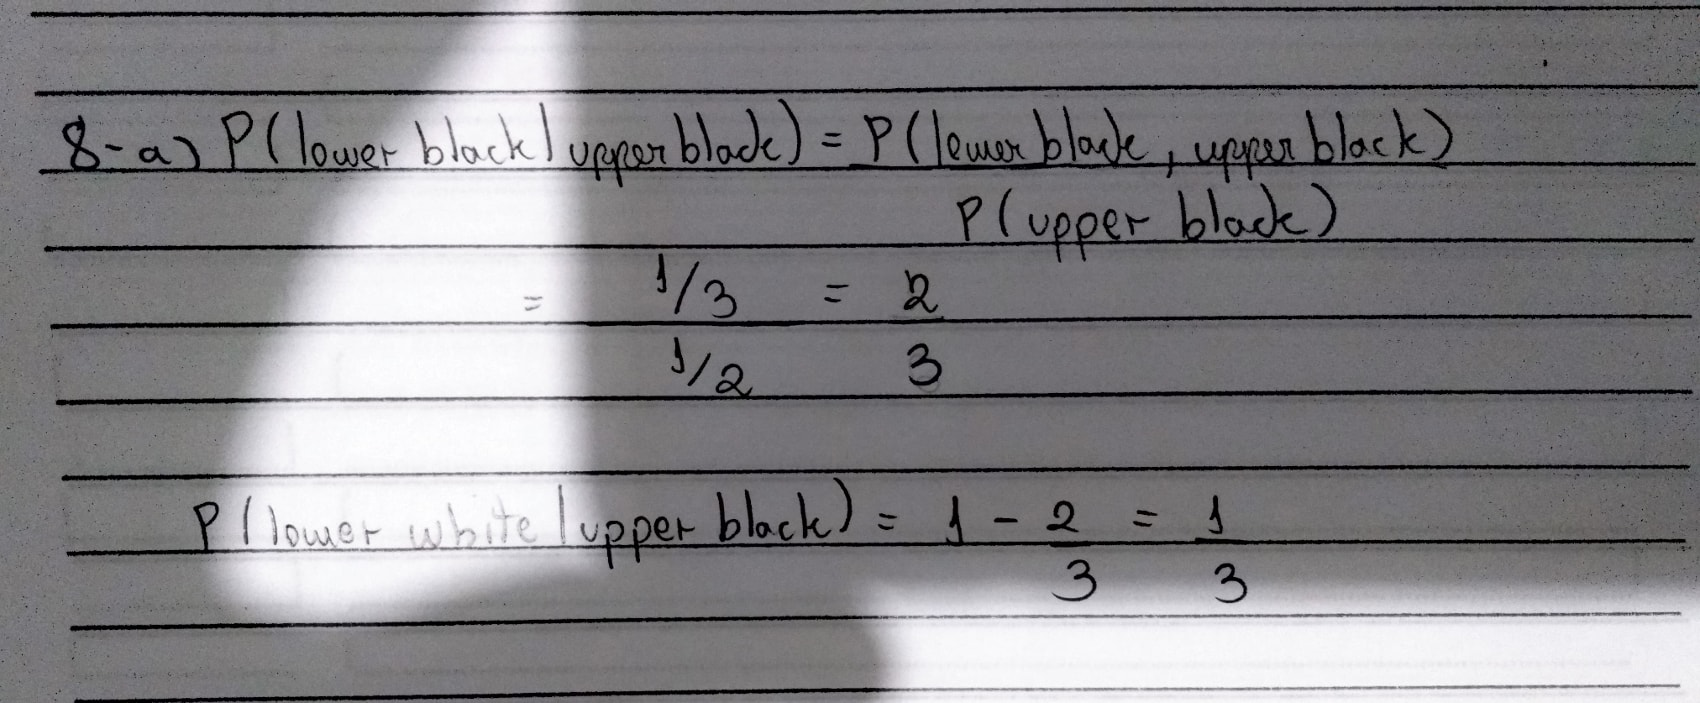
\includegraphics[width=0.8\textwidth]{images/6.jpg}
	      \end{figure}
	\item
	      \begin{enumerate}
		      \item \(\mathcal{P}_z = \{1/2, 1/2\}\)
		            \[\mathcal{P}(z = 0) = \mathcal{P}(x = 0) \mathcal{P}(y = 0) +\mathcal{P}(x = 1) \mathcal{P}(y = 1)\]
		            \[\mathcal{P}(z = 0) = \mathcal{P}(x = 0) \frac{1}{2} +\mathcal{P}(x = 1) \frac{1}{2}\]
		            \[\mathcal{P}(z = 0) = \frac{p + 1 - p}{2} = \frac{1}{2}\]

		            \[I(Z; X) = H(Z) - H(Z|X) = 1 - 1 = 0\]
		      \item For genral \(p\) and \(q\) we have
		            \[\mathcal{P}(z = 0) = \mathcal{P}(x = 0) \mathcal{P}(y = 0) +\mathcal{P}(x = 1) \mathcal{P}(y = 1)\]
		            \[\mathcal{P}(z = 0) = pq + (1 - p)(1 - q)\]

		            Consequently,

		            \[\mathcal{P}(z=1) = 1 - pq - (1 - p)(1 - q) = p(1 - q) + q(1 - p)\]

		            Therefora, for general \(p\) and \(q\), we have \(\mathcal{P}_z = \{pq + (1 - p)(1 - q), p(1 - q) + q(1 - p)\}\).

		            For the mutual information, we have:

		            \[I(Z; Y) = H(Z) - H(Z | X) = H(pq + (1-p)(1-q)) - H(q)\]
	      \end{enumerate}
	\item
	      \begin{itemize}
		      \item Handmade exercise.
		            \begin{figure}[H]
			            \centering
			            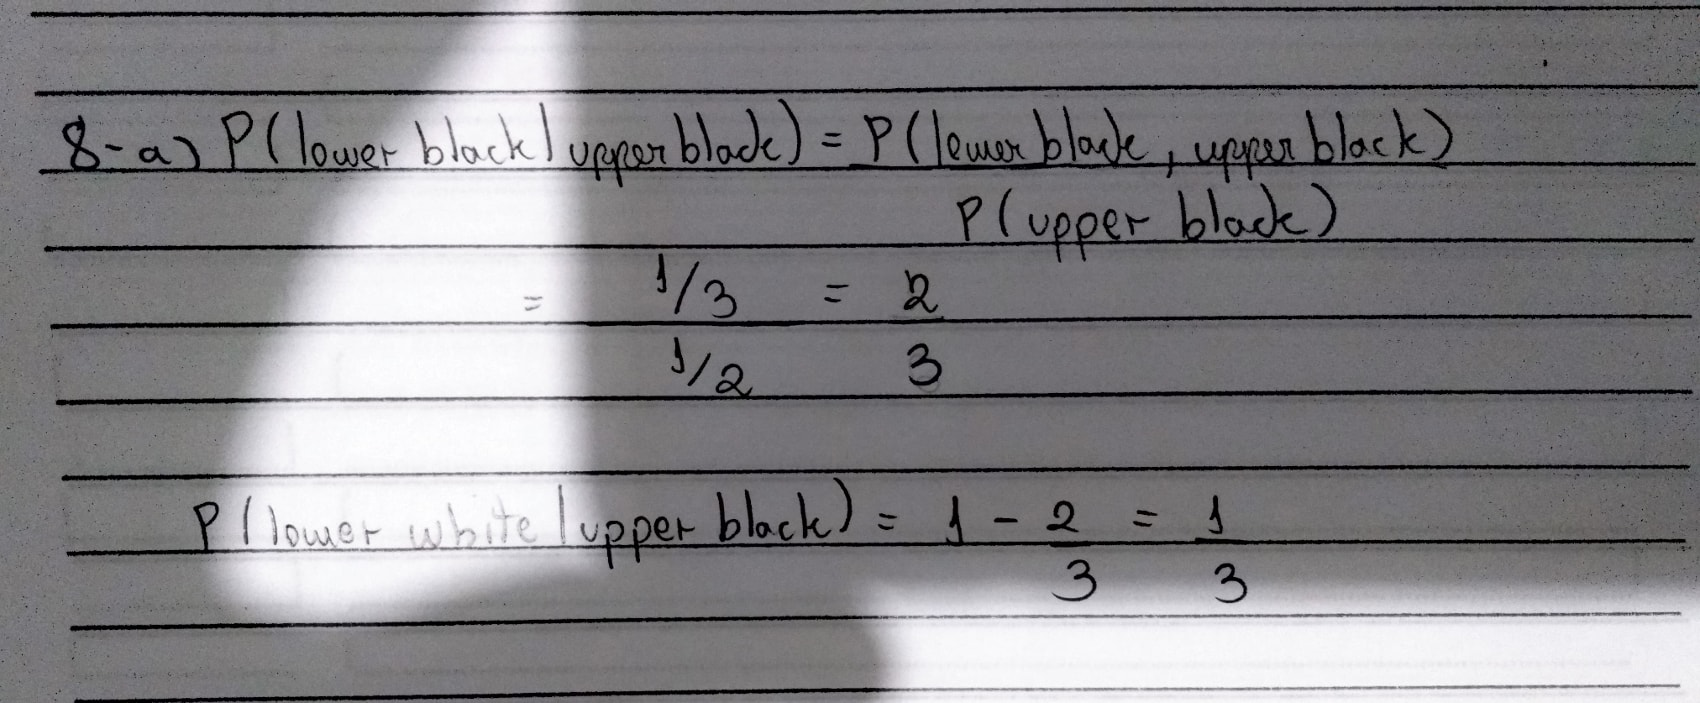
\includegraphics[width=0.8\textwidth]{images/8.jpg}
		            \end{figure}
		            As we can see, the probability that the lower face of the card is white is \(1/3\) and the probability that the lower face of the card is black is \(2/3\).
		      \item Yes, it certainly does. Since the probability distribution over the color of the upper or lower face of a random selected card is uniform, we can say that both \(H(U)\) and \(H(L)\) are qual to 1 bit. If we know the color of the upper side of the card, we have:

		            \[H(L | U = black) = H(L | U = white) = H_2(1/3, 2/3) = -\frac{1}{3} log \frac{1}{3} - \frac{2}{3} log \frac{2}{3}\]

		            \[H(L | U) = P(U = black) H(L | U = black) + P(U = white) H(L | U = white)\]
		            \[H(L | U) = \frac{1}{2} (log 3 - \frac{2}{3}) 2\]
		            \[H(L | U) = (log 3 - \frac{2}{3})\]

		            With this value, we can finally compute the mutual information \(I(L;U) = H(L) - H(U | L) = 1 - log 3 + \frac{2}{3} = \frac{5}{3} - log3\). So we can say that learning the color of the upper side of the card gives a non zero amount of bits of information about the color of the lower side of the card.
	      \end{itemize}
\end{enumerate}

\bibliography{sample}

\end{document}
